%----------------------------------------------------------------------------------------
%	PREPROCESSING PIPELINE AND DATA SET CREATION
%----------------------------------------------------------------------------------------
\section{Preprocessing and data set creation}
\label{ch:Dataset}

In this chapter, the different preparatory steps for the recorded data are described, including the creation of a data set which is usable for any machine learning or computer vision approach to analyze the image data.

In~\ref{sec:Preprocessing}~\nameref{sec:Preprocessing} the data is assessed and simplified for any further processing. The second section,~\ref{sec:AutomaticFeatureExtraction}~\nameref{sec:AutomaticFeatureExtraction}, deals with the creation of feature scripts that were researched and implemented for an automatic recognition of single features.
The results were combined in an application which is described in detail in~\ref{sec:LabelApp}~\nameref{sec:LabelApp}. In~\ref{sec:ManualLabeling}~\nameref{sec:ManualLabeling}, the process of hand-labeling the images for their feature class with the label application is described, followed by a section analyzing the results and comparing the overall agreement of the labelers. The last section~\ref{sec:AsparagusDataSet}~\nameref{sec:AsparagusDataSet} concludes with the creation of the final data set, used for the later training of the neural networks and other approaches to detect the label of a spear from its three images.


\subsection{Preprocessing}
\label{sec:Preprocessing}

Before implementing any approach that allows to predict a label to an asparagus spear, the recorded image data has to go through multiple preprocessing steps. In the following, these are elaborated in detail. \footnote{\url{https://github.com/CogSciUOS/asparagus/blob/master/preprocessing/perform\_preprocessing.py}}

\bigskip
As described in~\autoref{sec:DataCollection}, each asparagus can be found in three pictures, one in each of the three positions – left, center and right. The image names are used to combine the three relevant images and determine in which position the asparagus is captured. The images are cut into three pieces and renamed in a way that makes it clear which images belong together. Each asparagus gets a unique identification number and the three perspectives are denoted with textit{a} for left, textit{a} for center, and textit{a} for right. For example, the texttt{image 42\_b.png} is the center image of the asparagus spear with the identification number 42. 

Another step is to remove the background of the image. As the conveyor belt is blue, there is a high contrast to the bright asparagus spears which aids in the background removal (see \autoref{fig:PreprocessingCropping}). Hence, it is possible to mask the asparagus spear using the hue of the HSV representation of each image. All pixels with a blue hue and very dark regions are marked as background through threshold limitation of the value component. This is particularly important for the automatic feature extraction (see~\autoref{sec:AutomaticFeatureExtraction}).

\begin{figure}[!ht]
	\centering
	\includegraphics[scale=0.4]{Figures/chapter03/preprocessing_example.png}
	\decoRule
	\caption[Example Asparagus Images (2)]{\textbf{Example Asparagus Images (2)}~~~The figure shows three unprocessed images that depict an asparagus from three angles (see also \autoref{fig:ExampleImagesAnna}). The respective spear is left in the first image, in the center of the second image, and right in the third one.}
	\label{fig:PreprocessingExamples}
\end{figure}

\begin{figure}[!ht]
	\centering
	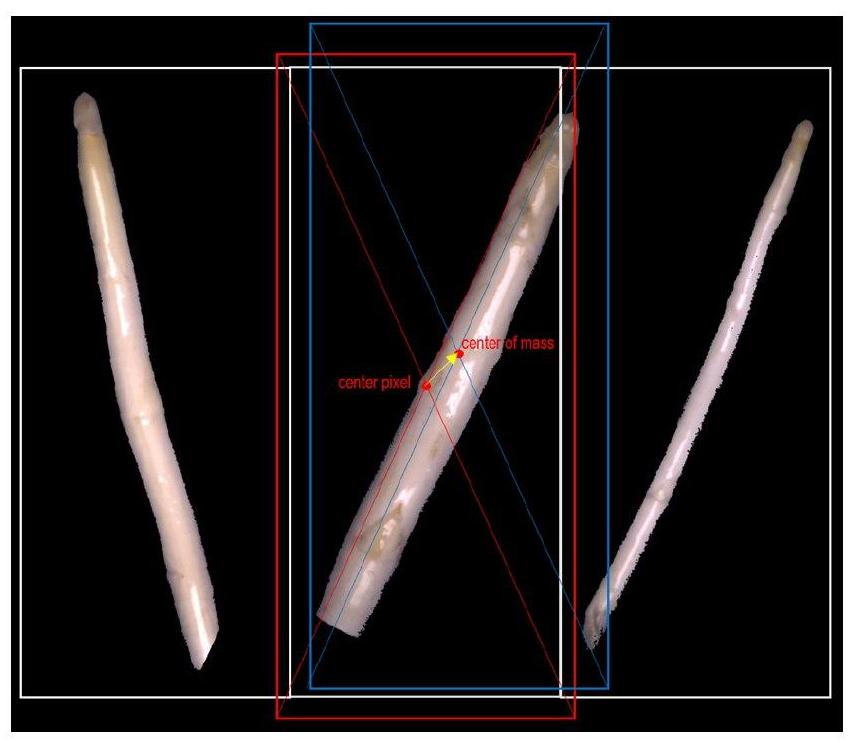
\includegraphics[scale=0.4]{Figures/chapter03/preprocessing_cropping.png}
	\decoRule
	\caption[Cropping Based on Center of Mass]{\textbf{Cropping Based on Center of Mass}~~~The depiction shows the effect of moving the cropping window (red) to a new location (blue) by moving it's center to the center of gravity (yellow arrow). The approach is applicable for all three images given that the initial coordinates are set to the respective positions.}
	\label{fig:PreprocessingCropping}
\end{figure}

\bigskip
To combine the three perspectives of each asparagus spear, the cropping regions are set to three patches that are a little larger than the compartments of the conveyor belt. They are located such that they cover the piece of interest. As it has been found that some tilted spears span across the borders between the coneyer compartments, the cropping window in the images was moved. The new coordinates are determined by shifting the center of the current cropping box horizontally to the center of mass of the contained foreground pixels (see \autoref{fig:PreprocessingCropping}).Repeating the procedure in a second iteration can further improve the result. As this is the case for few examples only we refrained from doing so to increase processing speed. Small parts of the neighboring depiction potentially end up in the region of interest as well. These remainders are removed by masking out all pixels that do not belong to the main blob of connected pixels.

\bigskip
To further reduce the variance the asparagus spears are rotated upwards to reduce the variance in angle. The rotation angle is achieved by binarizing the image into foreground and background pixels, calculating the centerline as the mean pixel location along the vertical axis, and fitting linear regression to the centerline pixels.

\bigskip
Another preprocessing step, which generates an additional set of images, is quantization using a common color palette. It was mainly employed to allow for the computation of meaningful color histograms.\footnote{ The number of colors in the original 24 bit RGB colorspace is too large to use them as bins for the histograms: The low number of pixels per bin would not allow for meaningful statistics. By reducing the number of colors one solves this problem.}  An appropriate palette and the respective mapping of RGB values to palette colors is determined using clustering in color space. First, a set of RGB tuples is collected by adding pixel values of 10000 asparagus spears. Second, the resulting list of RGB tuples is converted to an image such that a palette can be determined using standard tools for quantization. In the last step a clustering algorithm is employed that determines the position of cluster centers while maximizing the maximal coverage. The resulting cluster centers can be displayed as a list of RGB values which represent the color palette.\footnote{Here we used a standard implementation for image quantization that employs a maximal coverage algorithm ~\citep{pil_quantization}. An optimal solution to the problem of maximum coverage relates to the challenge of distributing a given number of facilities such that they cover the largest possible area of the sample space ~\citep{zarandi2011large}. One can interpret the centers of named facilities as cluster centers. For each data point (here: pixel), the closest cluster center is determined and the respective value attributed. This means the data is quantized.} The color palette is used for quantization of the images: Each image of the downscaled data set is transformed to the palette representation. Visual inspection shows little quality loss such that it can be assumed that the relevant information for image classification is well preserved.

\bigskip
Several additional collections of preprocessed images are computed based on the data without background. This holds for downscaled versions as well as for a version that contains the asparagus heads only. To compute the latter, the images are padded to avoid sampling outside of the valid image boundaries and the uppermost foreground row is detected. Subsequently, the center pixel is determined and the image is cropped such that this uppermost central pixel of the asparagus is the center of the uppermost row of the snippet. The resulting partial images of asparagus heads are rotated using the centerline regression approach described above. The approach has proven reliable and the resulting depictions are used to train a dedicated network for head related features (see~\autoref{subsec:HeadNetwork}).


\subsection{Automatic feature extraction}
\label{sec:AutomaticFeatureExtraction}

In this chapter, the different automatic feature extraction methods will be described, alongside with the results that were achieved and future steps that could be taken to improve the results further. For each feature detection method, the images with removed background are used. 

\bigskip
According to the producer of the Autoselect ATS II, the software currently on the market uses very similar methods. This gives us reason to believe that the classical methods might not be adequate to yield a better classification than the current status quo.

The results vary greatly between the different feature extraction methods. While the functions to detect the width and length and whether the asparagus is violet or bent are good enough to be integrated into the hand-label app (see~\autoref{sec:LabelApp}), other features turned out to be more difficult.


\subsubsection{Length}
\label{subsec:Length}

The length detection uses a pixel-based approach. It counts the number of rows from the highest to the lowest pixel that is not a black background pixel and therefore not zero. The asparagus is rotated upwards, as described in~\autoref{sec:Preprocessing}. This is done to improve the results, as the rows between the highest and the lowest pixel are counted and not the pixels themselves. This technique is a simplification, which does not represent curved asparagus very well, because it will have a shorter count than it would have if the pixels were counted along the asparagus spear. However in reality, there are not a lot of asparagus spears close to the decision boundary between a fractured spear and a whole spear. Usually, the asparagus is harvested a few centimeters longer than necessary and then cut to the desired length. The only asparagus shorter than that length are the ones that break during the sorting process. Moreover, if they break, they generally break closer to the center of the asparagus rather than at the ends. Therefore, the difference in length detection does not matter for our classification.

\bigskip
All in all, by visual inspection the length detection yields good results that are very helpful for the hand-label app. The next step would be to train a decision boundary that determines which number of pixels should be the threshold to differentiate between fractured and not fractured. At first, we tried to calculate this threshold by finding a conversion factor from pixel to millimeter, as we know the cut off in millimeters. But this approach appeared to be more difficult than anticipated, because the conversion factor varies in the different image positions. This problem only became apparent after the asparagus season had ended, for which reason we could not reproduce the camera calibrations in retrospective in order to take well-measured images, for example from a chessboard pattern. Accordingly, the threshold needs to be deduced from the data manually or learned with a machine learning approach.

\subsubsection{Width}
\label{subsec:Width}

The width detection uses a very similar approach as the length detection. It takes the pixel count from the left-most to the right-most pixel in a certain row as a width measure. But in contrast to the length, the width was measured at several image rows from which the mean width was taken. Since the width detection works reliably, it is integrated in the hand-label app (see \autoref{sec:LabelApp}).

\bigskip
The algorithm operates as follows: Firstly, the images are binarized into foreground and background, which means setting all pixels that are not zero, and therefore not background, to one. After that, the uppermost foreground pixel is detected and the length is calculated with the length detection function as described above. The length of the asparagus is used to divide it into even parts. This is done by determining a start pixel and dividing the remaining rows that contain foreground pixels by the number of positions one wants to measure at. This way several rows are selected in which the number of foreground pixels is counted. One can interpret each row as a cross-section of the asparagus, therefore the number of foreground pixels is a direct measure for the width. Then, the mean of these counts is calculated and used as the final width value. As the head of the asparagus can be of varying form and does not represent the width of the whole asparagus well, it is excluded from the measure. This is done by selecting a start pixel below the head area instead of naively choosing the uppermost pixel. To be precise, the start pixel is chosen 200 pixels, which corresponds to roughly 25 mm, below the uppermost pixel in order to bypass the head area with certainty. As described in the section \nameref{subsec:Length}, also the width detection might lead to slightly different outcomes on curved asparagus spears than the true values. Again, this difference is regarded as irrelevant in our case.

\subsubsection{Rust}
\label{subsec:Rust}

The rust detection finds all pixels that fall in the range of RGB values that correspond to the color brown. Those pixels are counted and normalized by the maximal number of possible pixels that could be rusty, namely the number of foreground pixels. Since it is impossible that the whole asparagus is rusty and hence that all the foreground pixels fall into the relevant range of RGB values, this normalization yields small numbers as results. To give an example, an output value of 0.13 is already considered moderately rusty. The lower and upper bound for the RGB values are set to $[50,42,30]$ and $[220,220,55]$, respectively. That means, all pixels that have a red value between 50 and 220, a green value between 42 and 220, and a blue value between 30 and 55 are considered to be rust.

\bigskip
Visual inspection shows that the rust detection algorithm works well to detect rusty areas and barely misses any rusty parts. Setting a threshold for the number of pixels needed to be classified as rusty still turns out to be difficult. Only clusters of brown pixels are a reliable indicator for rust.  Many pixels with a brown color distributed over the whole spear are not supposed to be classified as rust. To make this intuition more clear, it could be the case that two asparagus spears have the same number of brown pixels, but in one case they are all connected building a cluster and in the other case they are evenly distributed over the whole asparagus spear. That would mean that, although both yield the same output value, only the asparagus with the connected region should be considered as being rusty. However, it should be mentioned that this is merely an artificial example to display one draw-back of the implementation. In reality, it is very unlikely that an asparagus spear has a large number of brown pixels that are not in fact rust. Nevertheless, it remains unsolved to set a robust threshold that works well on the whole data set.

\bigskip
One problem that cannot be solved algorithmically is dirt in the sorting machine. If the machine is not cleaned thoroughly and regularly, dirt can be falsely classified as rust because it often falls in the same color range. Another problem can be a change of lighting when taking the images. Both issues can be controlled for, but have to be communicated well to the farmers.


\subsubsection{Violet}
\label{subsec:Violet}

In a simple approach to measure whether an asparagus spear is violet or not, color hues are evaluated. More precisely, this strategy is based on evaluating histograms of color hues that are calculated for foreground pixels of the asparagus images after converting them to the HSV color space. Pale pixels are removed from the selection by thresholding based on the value component of the HSV representation. Finding the optimal threshold has proven difficult because of named subjectivity in color perception. A threshold of 0.3 for the value component is considered a good compromise: If applied, white and slightly rose pixels are masked out. All three perspectives are taken into account to compute a single histogram per asparagus spear. A score is calculated by summing up the number of pixels that lie within the violet color range. A second threshold is used as the decision boundary for violet detection. The direct and intuitive feedback in the hand-label app showed the relation between varying thresholds and the prediction. It could be seen that lowering the threshold also means that the feature extractor becomes more sensitive at the price of a reduced specificity. Best overall matches (accuracies) with the subjective perception are found for very low thresholds. In many cases, however, measurements based on this definition of violet do not match the attributed feature label.

Hence, another sparse descriptor is derived from the input images. Instead of setting thresholds for pale values and calculating the histograms of color hues, this approach relies directly on the colors that are present in the depiction of an asparagus spear. As the 24 bit representations contain a vast amount of color information in relation to the number of pixels, it is, however, unfeasible to use these as input. Instead, the color palette images can be used. Histograms of palette images can serve as the basis to define the feature violet in a way that captures more of the initial color information. At the same time it is simple and understandable enough to allow for customizations by users of sorting algorithms or machines. As a consensus regarding such an explicit definition is hard to achieve and somewhat arbitrary, the descriptor is used to learn implicit definitions of the feature through examples (see~\autoref{subsec:FeatureEngineering}).

\bigskip
The lack of a formal definition for violet asparagus spears has proven to be a major challenge to approaches of measuring this feature. It has been shown that directly measuring whether an asparagus spear is violet heavily depends on the definition of this feature. It is to mention that color impression is highly subjective across and even within subjects ~\citep{luo2000review}. Effects of meta contrast that make minor variations in color more visible arguably affected the attribution of labels when many similar spears were assessed in succession ~\citep{reeves1981metacontrast}. Hence, machine learning approaches that are trained on human labeled data appear to be more promising. Using them can help to find the definition that generalizes best over varying color perceptions and retrieve objective rules to measure the degree to which an asparagus is violet.



\subsubsection{Curvature}
\label{subsec:Curvature}

Multiple curvature scores can easily be computed based on regression fits to the centerline of an asparagus spear. For example, the parameters of linear or polynomial regression can be interpreted as a description of how bent an asparagus spear is. 

\bigskip
Deriving sparse descriptions is based on a two-stage approach. In the first stage, the centerline of an asparagus spear is computed because it is considered to be a good description of the curvature of asparagus spears. In each image the asparagus spear is roughly vertically oriented. This means that also for bent spears the head relies within the top center of the image (see \autoref{sec:Preprocessing}). The centerline is computed by binarizing the image into foreground and background and computing the mean of pixel locations along the vertical axis (i.e.\ for each row). The resulting binary representation shows a single pixel line. It serves as the input to the second stage of curvature estimation.

In the second stage, curves are fit to the pixel locations of the centerline. For a simple score, linear regression is employed and the sum of squared errors is thresholded and interpreted as a curvature score. This score is small for perfectly straight asparagus spears and increases the more bent an asparagus is. As an S-shaped asparagus is arguably perceived as bent even when the overall deviations from the center line are small, a second descriptor was computed as the ratio between the error of a linear fit and polynomial regression of degree three. Thresholding values and employing a voting scheme for the results for all three perspectives yields a rule to measure curvature (e.g.\ at least one of the three perspectives indicates that the asparagus is bent). However, it has again proven difficult to set thresholds appropriately to reliably capture the visual impression. Hence, another sparse representation was calculated by dividing the spears into several segments and fitting linear regression to each segment. A \acrfull{mlp} was trained on the resulting 18 angles per asparagus (see~\autoref{subsec:FeatureEngineering}).

\bigskip
Calculating a score for curvature is fast and efficient. While the respective approach is suitable to define curvature, it does not necessarily meet up with the subjective perception of how bent an asparagus appears. Just like histograms of palette images, curvature scores are the results of feature engineering: The use of extensive domain knowledge to filter relevant features~\citep{zheng2018feature}. They can serve as an input to a machine learning approach that maps this sparse representation to the target categories (see~\autoref{subsec:FeatureEngineering}).


\subsubsection{Flower}
\label{subsec:Flower}

The implementation of the flower detection function turned out to be difficult to realize. Several approaches have been tested, but none of them generated sufficiently good results. Two main notions were tried. The first approach uses the shape of the head as an indicator for a flower. The idea is that asparagus spears with a flowery head exhibit a less closed head shape. In other words, the head looks less round and has no smooth outline, but shows fringes. The second approach focuses on the structure within the head. Supposedly, asparagus with flowery heads exhibit more edges and lines in the head area. In both cases, it is challenging to find a way to discriminate between asparagus with and without flowery heads. One reason for that is the poor resolution of the camera that is installed in the sorting machine. With a pixel to millimeter ratio of around four to one, it is even difficult to detect flowers with the human eye. Likewise, the current software in the machine struggles greatly with the classification of this feature as well.


\subsection{The hand-label app: A GUI for labeling asparagus}
\label{sec:LabelApp}

Providing a sufficiently large data set that contains information about target categories is one of the major non-algorithmic challenges in the application of machine learning for classification tasks~\citep{al2018labeling}. In many cases, however, the respective labels are missing. This is especially problematic if traditional supervised learning methods such as feed forward \acrshortpl{cnn} are employed: If the variance in the input images is high, a very large number of samples is required~\citep{russakovsky2015imagenet}. 

\bigskip
The options to reduce the variance and hence the need to attribute labels to a very large number of samples are limited. We employed preprocessing and manual feature engineering and employed strategies on the algorithmic domain such as unsupervised and semi-supervised learning (see~\autoref{sec:SemiSupervisedLearning} and ~\autoref{subsec:FeatureEngineering}) as it promises to limit the required number of labels. Nonetheless for training and more importantly performance evaluation of machine learning models a substantial amount of labels are required. Otherwise quality metrics such as accuracies, sensitivity and specificity cannot be calculated. Hence labels had to be manually attributed.

\begin{figure}[!htb]
	\centering
	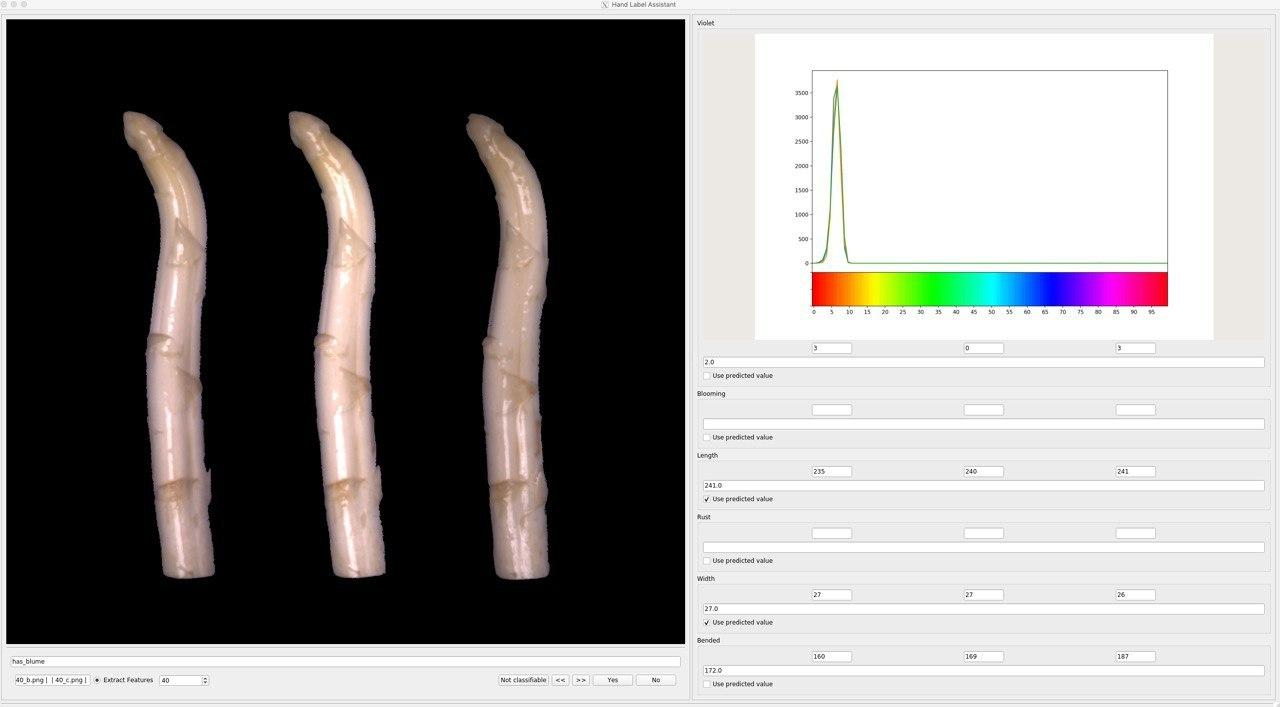
\includegraphics[scale=0.3]{Figures/chapter03/labelapp_example.png}
	\decoRule
	\caption[The Labeling Dialog of the Hand-Label App]{\textbf{The Labeling Dialog of the Hand-Label App}~~~The depiction shows the main dialog used for labeling. In the left part you can see all three available images (perspectives) for the asparagus with the ID 40. The current question that targets at one of the features of interest is displayed in the area below the images. They are phrased such that the user can answer them with yes or no using the respective buttons or keyboard controls. On the right side you can see the results of the automatic feature extraction. The upper right panel shows the histogram of color hues.}
	\label{fig:LabelAppGUI}
\end{figure}

Annotating labels manually requires plenty of effort. ``Data set annotation and/or labeling is a difficult, confusing and time consuming task’’~\citep[p.~2]{al2018labeling}. Human performance is often acknowledged as the baseline or ``gold standard’’ that image classifiers are evaluated by. Hence, in many scenarios data is labeled by humans such that machine learning algorithms can be applied. This holds especially for image classification.\footnote{For example the performance of GoogLeNet is compared to human level performance using the ImageNet data set~\citep{russakovsky2015imagenet}.} In the present case some features were reliably measurable by means of classical computer vision algorithms (e.g.\ the width or the length). For features such as a flower or the evaluation whether or not a spear is affected by rust, this has proven to be difficult (see~\autoref{subsec:Rust}). Considering the amount of data that could potentially be labeled, a custom interface is required that allows for time efficient attribution of labels.

\bigskip
A custom application was built that comprises two user interfaces: A startup window that allows for a preview of asparagus images and the attributed labels (represented by Ui\textunderscore Asparator) and the main labeling interface (Ui\textunderscore LabelDialog) (see \autoref{fig:LabelAppDiagram}). Using the labeling interface is possible only after the user selects the source folder of images and specifies or loads a file that contains the attributed labels. This ensures that the file paths for input and output are set. A dictionary that maps indices to images can be parsed from file names and the minimum index is determined. As such, the label dialog and the respective controller class always reside in a valid initial state. For labeling, the user answers questions that are displayed alongside the images that depict each asparagus spear from three perspectives. This can be done using the respective buttons or the arrow keys (see \autoref{fig:LabelAppGUI}). The result is saved and the next question will automatically appear upon answering. 

Automatic feature detection can be selected as an alternative for manual labeling for specific features. The result is displayed and saved to a file. This flexible approach was chosen as it is initially unclear and disputed in how far automatic feature extraction yields results that meet up with the individual, subjective perception. It also allowed to improve automatic feature extraction methods and to develop a direct intuition for the relation to the data. On top of that, it has proven to be useful for debugging automatic feature extraction methods that initially failed for some images.

\bigskip
The development of the app was accompanied by three major challenges. First, handling a large data set of several hundred gigabytes that is accessible in a network drive. Second, changing requirements that resulted from group decision processes with respect to automatic feature extraction as well as from unforeseen necessities in (parallel) preprocessing. This required substantial changes of the initial architecture and the reimplementation of parts of the code. The third challenge is related to the question of the handling of internal states of the app. The latter may be further explained in the following. 

Internal states of the app are handled such that it is possible for the user to navigate into invalid states for which no images are available. Note that preprocessing was done such that each asparagus spear has a unique identification number and a specifier for perspectives textit{a}, textit{b} and textit{c} in it’s filename. While generally the identification numbers are in a continuous range from zero to n, some indices are missing. As preprocessing jobs were scheduled to run in parallel and preprocessing failed for few corrupted files, it has proven almost inevitable to end up with some few missing indices although a dictionary of input filename and output filename was passed to each grid job. In addition, the large amount of data did not allow to save all files in a single directory. In summary, this means that one could not simply iterate over asparagus identification numbers (represented by the state of a spin box in the user interface), determine the file path, and display the related images. Instead, parsing file names from a slow network drive is necessary which requires limiting the number of selected images. As GUI elements such as spin boxes and keyboard controls allow for setting an integer, and it was a requirement that this integer relates to the asparagus identification number, one ends up with the following situation: Either one prevents that the asparagus identification number is set or incremented freely to a value that does not exist, or one allows to navigate into an invalid state. The latter solution was considered to be easier and thus implemented.\footnote{The earlier approach showed to have several implementation specific drawbacks. Note for example that upon entering multiple digits in an input field, an event is triggered multiple times. Upon entering the value 10 for the asparagus identification number, one ends up with the value being set to 1 before being set to 10 where 1 relates to a potentially missing identification number. This means the user cannot freely enter IDs because setting them to certain values is impossible.} Hence, all cascades of methods of the app including preprocessing functions that require the respective images as an input were adjusted such that they can handle this case. 

\begin{figure}[!t]
	\centering
	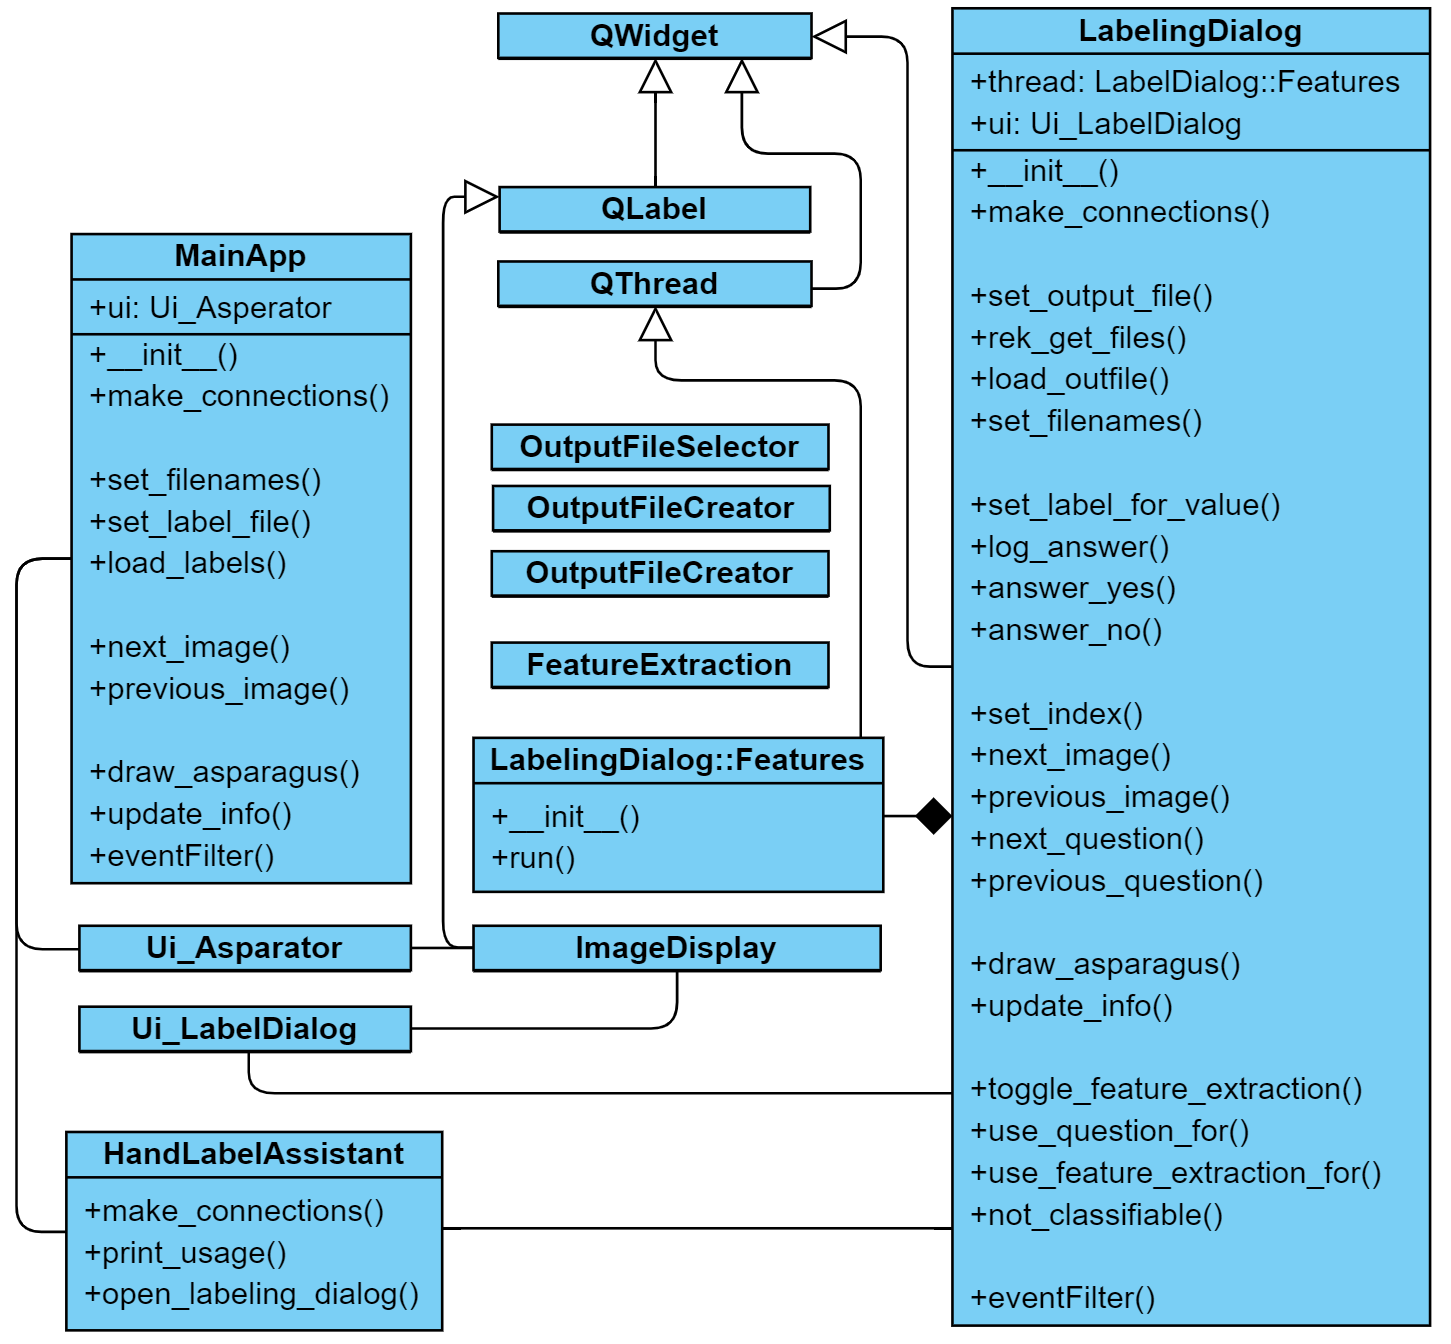
\includegraphics[scale=0.3]{Figures/chapter03/label_app_diagram.png}
	\decoRule
	\caption[UML Diagram for the Hand-Label App]{\textbf{UML Diagram for the Hand-Label App}~~~The depiction shows the class diagram for the hand-label app in UML (unified modeling language).}
	\label{fig:LabelAppDiagram}
\end{figure}

The app is implemented using the PyQt5 framework\footnote{see \url{https://pypi.org/project/PyQt5/}} while coarsely following the model, view controller principle. Model and controller are not strictly separate and thus no distinct model class or database is used. Instead the labels are managed as a Pandas DataFrame and serialized as a csv-file. Upon state change (i.e.\ index increment), images are loaded from the network drive that is mounted on the level of the operating system. The views are designed using QtDesigner. Four manually coded classes are essential for the architecture of the app: (1) The class HandLabelAssistant in which the PyQt5 app is instantiated, (2) the controllers MainApp and (3) LabelingDialog as well as (4) Features which is member class of the latter. Features is of type QThread and represents the API to the automatic feature extraction methods in FeatureExtraction. Ui\textunderscore Asparator, UiLabelDialog and classes for file dialogs represent the views. A class ImageDisplay is required to display images with the correct aspect ratio. \autoref{fig:LabelAppDiagram} shows the UML class diagram alongside methods and attributes that are considered relevant to understand the architecture of the app. 

\bigskip
Developing a custom app for the labeling process required substantial time resources. However, it was found that existing solutions did not meet the specific requirements. Our custom hand-label app allowed us to attribute labels to more than 10000 asparagus in a manageable amount of time. Details of the manual labeling process are described in the next section.


\newpage

\subsection{Manual labeling}
\label{sec:ManualLabeling}

In this section, the process of manually labeling the data with the help of the hand-label app is laid out. This includes the labeling criteria which allocate each spear to a single quality class, the practice of manually labeling the preprocessed data for its features, the outcome of the labeling process, and one approach to measure the agreement of the manual labeling.

\bigskip
The images were labeled by all members of the group. As none of the team members were experts in asparagus labeling, a general guideline for the labeling had to be established. The guideline was written in accordance with the owner of the asparagus farm Gut Holsterfeld, Mr. Silvan Schulze-Weddige. He was consulted in all questions regarding the labeling of the asparagus. 

General challenges in the manual labeling in front of a computer screen, including the respective image quality, and the variance in the agreement of the project members were expected from the start. As the task relies on the subjective view of individual humans, opinions about the affiliation to one asparagus class label can diverge. By consulting Mr. Schulze-Weddige on difficult decision-making for the team, it became clear that some examples are difficult to classify even for experts. 

To tackle the issue and to have an overview of the general agreement of the labeling between group members, a measure was applied, namely the Kappa Agreement. The Kappa Agreement was used to assess the degree of accordance in labeling between the single members and monitor how the labeling agreement developed during the manual labeling process. 


\subsubsection{Labeling criteria}
\label{subsec:SortingCriteria}

The class label of an asparagus spear is decided by several factors, ranging from its shape to its color. Put together, these single features give the class label, that attributes an asparagus to a quality class (for a description of the quality classes, see \autoref{tab:AsparagusLabels}, and further \autoref{fig:LabelTree} on how the features decide the class label). As it was decided to label the images for their features rather than final class labels, the features were checked by the labelers. Even though the chosen features closely resemble the class labels defined by Gut Holsterfeld, they are different and should not be confused with one another. The images are displayed with the hand-label app and the features are as follows: fractured, hollow, flower, rusty body, rusty head, bent, violet, very thick, medium thick, thick, thin, very thin. Further, images that could not be classified thoroughly were labeled as ``not classifiable’’ (e.g.\ when the spear is cut off the image).

\begin{wrapfigure}{!I}{0.35\textwidth}
  \begin{center}
    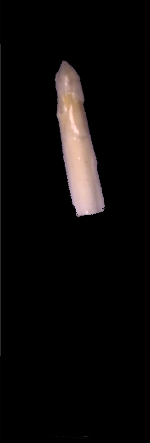
\includegraphics[width=0.15\textwidth]{Figures/chapter03/example_img_fractured.png}
  \end{center}
  \vspace{-15pt}
  \caption[Example Image Feature Fractured]{ \textbf{Feature Fractured}}
  \vspace{-20pt}
  \label{fig:ExampleFractured}
\end{wrapfigure}

In the following text, the different criteria for manually labeling the data images for their corresponding features are described. 

\bigskip
\textbf{Fractured}

An asparagus spear includes the feature fractured if it is broken, or if it does in any other way not fulfill the required length of 210 mm (see \autoref{fig:ExampleFractured}).

For this feature, the parameter length was used which is automatically calculated within the hand-label app.

\newpage

\begin{wrapfigure}{!I}{0.35\textwidth}
  \begin{center}
    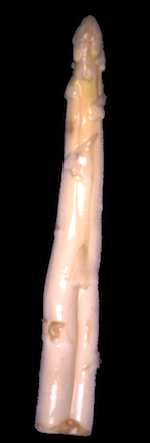
\includegraphics[width=0.15\textwidth]{Figures/chapter03/example_img_hollow.png}
  \end{center}
  \vspace{-15pt}
  \caption[Example Image Feature Hollow]{ \textbf{Feature Hollow}}
  \vspace{10pt}
  \label{fig:ExampleHollow}
\end{wrapfigure}

\textbf{Hollow}

The feature hollow indicates if the spear has a cavity inside.
This might be expressed by a bulgy center and a line running vertically along the spear’s body. Another, more distinct indicator is when the asparagus looks like two spears fused together, forming a single asparagus (see \autoref{fig:ExampleHollow}). A hollow asparagus can be confused with a very thick asparagus.

The feature can be easily checked when you have physical access to the asparagus. If the asparagus is actually hollow, it will have a hole at its bottom that is noticeable when turning the spear around. Unfortunately, this cannot be done when only looking at the spears from the side.

The feature hollow sometimes occurs without showing a clear line or obvious bulge at its center.

\begin{wrapfigure}{!I}{0.35\textwidth}
  \begin{center}
    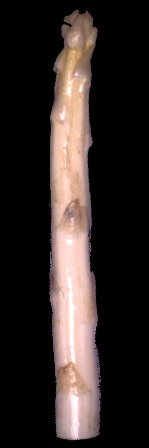
\includegraphics[width=0.15\textwidth]{Figures/chapter03/example_img_flower.png}
  \end{center}
  \vspace{-15pt}
  \caption[Example Image Feature Flower]{ \textbf{Feature Flower}}
  \vspace{-10pt}
  \label{fig:ExampleFlower}
\end{wrapfigure}

Therefore, there is a high risk of wrong classification.

\bigskip
\textbf{Flower}

The asparagus is graded as flower when the bud shape of the head is more developed (for more details, see the section \nameref{subsec:Flower}).

When a bud is in full bloom, it is clearly visible. However, it can be quite difficult to distinguish between an asparagus with clearly cut but closed petals and an asparagus that has just begun to develop a flower. It was decided to label the feature as absent when the asparagus does not clearly show the characteristic flower. With this decision, we assumed there to be less correspondence error between hand sorters.

\bigskip
\textbf{Rusty body}

If a spear has rust on its body, it is visible as a dark brown color.

\begin{wrapfigure}{!I}{0.35\textwidth}
  \vspace{-20pt}
  \begin{center}
    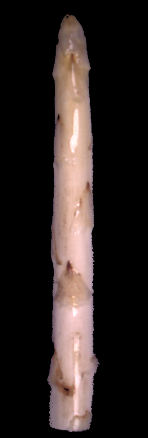
\includegraphics[width=0.15\textwidth]{Figures/chapter03/example_img_rustybody.png}
  \end{center}
  \vspace{-15pt}
  \caption[Example Image Feature Rusty Body]{ \textbf{Feature Rusty Body}}
  \vspace{-40pt}
  \label{fig:ExampleRustyBody}
\end{wrapfigure}

It often starts at the tips of becoming leaves or at the bottom part (see \autoref{fig:ExampleRustyBody}). The color is not to be confused with bruises, pressure marks, or a slightly yellow complexion, which can occur in a ripe asparagus. The latter coloring is neglected.
Rust is set to be present even when only the tip of a leaf shows a dark spot. Other brownish bruises are not classified as rust.

The feature rust is split into the sub-features rusty body and rusty head. In the case of rust being only on the body, it is removable by peeling.

\vspace{5cm}

\begin{wrapfigure}{!I}{0.35\textwidth}
  \vspace{-30pt}
  \begin{center}
    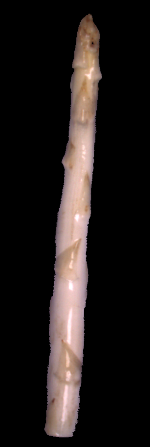
\includegraphics[width=0.15\textwidth]{Figures/chapter03/example_img_rustyhead.png}
  \end{center}
  \vspace{-15pt}
  \caption[Example Image Feature Rusty Head]{ \textbf{Feature Rusty Head}}
  \vspace{-10pt}
  \label{fig:ExampleRustyHead}
\end{wrapfigure}

\textbf{Rusty head}

If there is a dark spot on or close to the head region recognizable as rust, it is captured by this feature (see \autoref{fig:ExampleRustyHead}). The head part is usually distinct in shape and color from the body part of the asparagus.

In principle, the same guidelines which apply to the feature rusty body can be transferred here, with an explicit focus on the top part (until around 1 cm below the collar) of the asparagus. As rust at the top part of the spear cannot be removed without damaging the head, it is more decisive for the later categorization into a price class, if the head has rust. Therefore, this separation is of importance concerning the quality of a spear.

\bigskip
\textbf{Bent}

\begin{wrapfigure}{!I}{0.35\textwidth}
  \vspace{-10pt}
  \begin{center}
    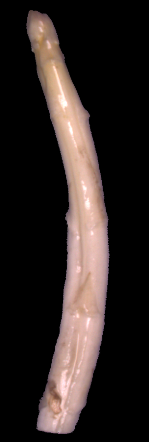
\includegraphics[width=0.15\textwidth]{Figures/chapter03/example_img_bent.png}
  \end{center}
  \vspace{-15pt}
  \caption[Example Image Feature Bent]{ \textbf{Feature Bent}~~~~~~~~}
  \label{fig:ExampleBent}
\end{wrapfigure}

An asparagus is categorized as bent, if the shape of the asparagus is curved and not straight (see \autoref{fig:ExampleBent}).

If it is only slightly curved but can otherwise be thought of as straight -- that means fitting next to other straight spears without standing out -- it is labeled as straight. 
If the spear looks close to the same on all three pictures regarding its shape, it might indicate that it is heavily bent and therefore cannot be turned on the machine’s conveyor belt.
The feature bent has a broader range of shapes where the asparagus is not obviously deformed but also not completely straight. An exception holds for S-shaped spears, which always count as bent.

\bigskip
\textbf{Violet}

The feature violet indicates whether an asparagus is of violet color.

\begin{wrapfigure}{!I}{0.35\textwidth}
  \vspace{-10pt}
  \begin{center}
    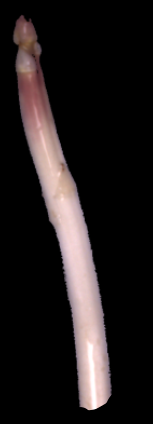
\includegraphics[width=0.15\textwidth]{Figures/chapter03/example_img_violet.png}
  \end{center}
  \vspace{-15pt}
  \caption[Example Image Feature Violet]{ \textbf{Feature Violet}}
  \vspace{-130pt}
  \label{fig:ExampleViolet}
\end{wrapfigure}

The shift of color from white to violet occurs most often around the head region - either at the tip of the head or just below the collar of the head region (see \autoref{fig:ExampleViolet}).
Here, the spear will darken further after it is labeled. Thus, even a slightly pink spear is labeled as being violet.

\vspace{8cm}
\textbf{Thickness and length}

\begin{wrapfigure}{!I}{0.35\textwidth}
  \centering
  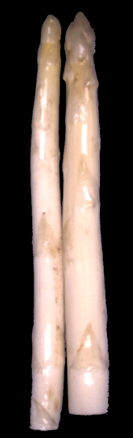
\includegraphics[width=0.15\textwidth]{Figures/chapter03/example_img_thick.png}
  \caption[Example Image Not Classifiable]{ \textbf{Feature Not Classifiable}}
  \label{fig:ExampleThickness}
\end{wrapfigure}

The thickness and the length are features hardly recognizable by view alone. Therefore, both measures are calculated from the computer-vision based feature extractions (see the sections \nameref{subsec:Width} and \nameref{subsec:Length}). The division into different categories of thickness can be inferred by the overall thickness of the spear.

The feature ‘very thick’ is attributed to asparagus that is more than 26 mm in width. Feature ‘thick’ corresponds to 20 - 26 mm, feature ‘medium thick’ to 18 - 20 mm, and feature ‘thin’ to 16 - 18 mm. Every asparagus with less than 16 mm in width is described with the feature ‘very thin’.

\bigskip
\textbf{Not classifiable}

%\begin{wrapfigure}{I}{0.3\textwidth}
%  \vspace{-20pt}
%  \begin{center}
%    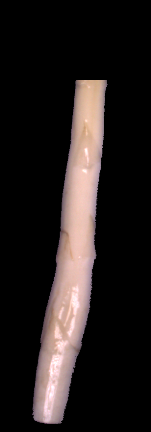
\includegraphics[width=0.15\textwidth]{Figures/chapter03/example_img_notclass}
%  \end{center}
%  \vspace{-15pt}
%  \caption[Example Image Feature Not Classifiable]{\\ \textbf{Feature Not Classifiable}}
%  \vspace{-20pt}
%  \label{img:ExampleNotClass}
%\end{wrapfigure}

Whenever the spear was unrecognizable, the head part of the spear was severed, two spears were present in one picture, the spear was cut off by the image, or other unusual circumstances occurred, it fell into the category of being unclassifiable (see \autoref{fig:ExampleThickness}).


\subsubsection{Labeling outcome}
\label{subsec:SortingOutcome}

In this section, the process and the results of the manual labeling are described.

The labels of all manually labeled images are stored in a csv-file, as shown in~\autoref{fig:CSVfileOverview}. The first entry is the image identification number. Every feature can be of value 0, value 1 or empty. Whenever a feature is present in an image, the value is set to 1. If the feature is absent, it is set to 0. For images labeled as not classifiable, all feature values remain empty. The image path to every of the three images for one spear is also saved in the label file in a separate column. After the labeling process, the individual csv-files with the labels are merged into one large \texttt{combined\_new.csv} file. The content of this file is later used for the classification of the data with the different approaches (see \autoref{ch:Classification}). It can be found in the study project’s GitHub repository.\footnote{see~\url{https://github.com/CogSciUOS/asparagus}}

\begin{table}[!hb]
	\centering
	\vspace{10pt}
	\resizebox{.75\linewidth}{!} & \textbf{Feature} & \textbf{\%} \\
		\hline
		hollow		&  3.3\%		& fractured			& 3.5\% 		\\
		flower		& 12.9\% 	& very thick 		& 4.0\% 		\\
		rusty body	& 45.5\% 	& thick 				& 29.1\%	 	\\
		rusty head~~~~~~~~~~~~~~~~~~& 14.7\% & medium thick & 18.7\% 	\\
		bent 		& 40.0\% 	& thin				& 17.9\% 	\\
		violet 		&  7.9\% 	& very thin 			& 30.3\% 	\\
		{} 	 		& {}  		& not classifiable~~~~~~~~~~~~~~& 2.1\%		\\
		\hline
	\end{tabular}%
	}
	\caption[Manual Labeling Feature Representation]{\textbf{Feature Representation in the Data Set} \\ In this table, the representation of each feature in the manually labeled 13319 asparagus samples is reported in \%.}
	\label{tab:FeatureRepresentation}
\end{table}

\begin{figure}[!ht]
	\centering
	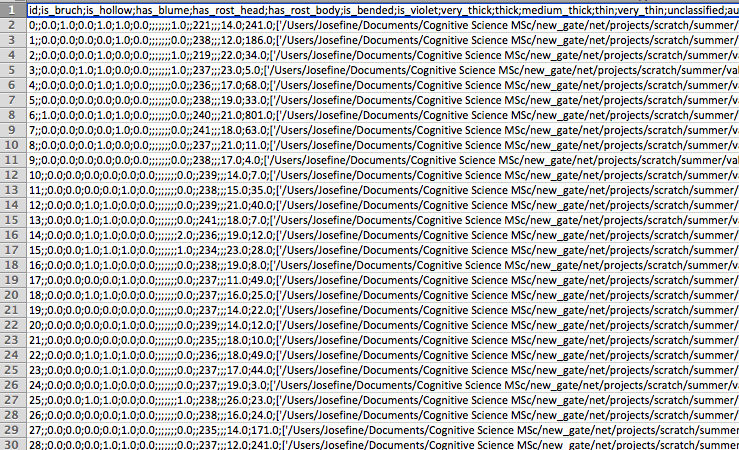
\includegraphics[scale=0.5]{Figures/chapter03/csv_overview.png}
	\decoRule
	\caption[Manual Labeling Output CSV-File]{\textbf{Label File}~~~The feature labels extracted by the manual labeling process were saved in a csv file. This image shows the beginning of the file \texttt{combined\_new.csv} in which all label files were later combined as one.}
	\label{fig:CSVfileOverview}
\end{figure}

\bigskip
The manual labeling lasted over the period of November 2019 to January 2020. A session usually consisted of 500 images, with an asparagus spear being viewed in three positions from the same angle. A session of labeling 500 images took between two and four hours. One minor factor sometimes influencing the time spent for labeling were difficulties with the external \acrshort{ssh} connection to the \acrshort{ikw} storage, as all images are stored on the university servers. The average time spent for labeling one asparagus is around 27 -- 48 seconds.

All in all, 13319 triples of images were labeled for their features. There is a large variance in the presence of the features in the data as can be seen in~\autoref{tab:FeatureRepresentation}. Of the acquired 13319 images, the feature most present in the data is rusty body with 45.5\%, followed by the feature bent with 40\%. Features whose representation is below 10\% include the features violet (7.9\%), hollow (3.3\%), fractured (3.5\%), and very thick (4\%). The feature not classifiable shows least presence with 2.1\%. 

It emerges that many features are only sparsely present in the data. This poses an imbalance in the data that is relevant for later classification tasks and the usage of the data set.

Further, every member of the group participated in the labeling but not everybody labeled the same number of images. Due to this circumstance, the labeling bias of certain members is more present in the data than of others.

The manual labeling was stopped when the amount of classified data exceeded 13000 samples. Reason for this is that we had reached our time limit for labeling samples.\footnote{To have an intuition of how much labeled data we might need, we found some of the suggestions in a blogpost helpful which can be visited at \url{https://machinelearningmastery.com/much-training-data-required-machine-learning/}. However, we did not find an exact number when to stop labeling.}


\subsubsection{Agreement Measures}
\label{subsec:AgreementMeasures}

When different annotators label data, it is indispensable to verify the degree of agreement among raters. In order to judge how consistently the data is labeled, several statistical methods (inter-rater-reliability) can be applied.

\bigskip
For the current purpose, different agreement measures, all implemented by scikit-learn, are used. The first is Cohen’s Kappa. It is seen as a more robust measure than a simple agreement percentage, such as a measure of true positives and true negatives, which was traditionally used for those cases~\citep{cohen1960coefficient}. Cohen’s Kappa is more robust, as the rate of agreement occurring by chance is included in the calculation. This method is applicable to compare the rating of two raters on a classification problem. The degree of agreement is always within $-1.0$ and 1.0 inclusive. The higher the Kappa value, the higher the agreement. Values around zero indicate no agreement and negative values indicate negative agreement which can be interpreted as systematic disagreement. Values between 0.41 - 0.6 are seen as moderate agreement, 0.61 -- 0.8 as substantial agreement, and everything above as almost perfect agreement. All scores below 0.4 are interpreted as unacceptable \citep{mchugh2012interrater}. 

Another statistical method used to measure the agreement is the F1 score. The F1 score is used for the evaluation of binary classification. It relies on both precision as well as recall of a test. An F1 score value lies between 0.0 and 1.0 -- the higher the F1 score, the higher the agreement.

Lastly, we calculated the accuracy measure. For a normalized accuracy score, the values lie between 0.0 and 1.0, and the best performance is 1.0. This measure returns the fraction of correctly classified samples. It is a less robust measure than Cohen’s Kappa score~\citep{mchugh2012interrater}.


\subsubsection{Reliability}
\label{subsec:Reliability}

In order to evaluate the degree of agreement of our data, we made agreement measures at two points in time.\footnote{for our API documentation see \\ \url{https://asparagus.readthedocs.io/en/latest/api/measure\textunderscore agreement.html}}

The first time, six different annotators assigned 13 features to images out of each class label group of sorted asparagus. We ensured that always two different annotators labeled the same set of images. The Kappa scores varied strongly between groups and features from $-0.03$ to 0.76, while the accuracy scores ranged from 0.49 to 1. We were surprised that the agreement scores are low, even though the raters gave the same label to many of the asparagus spears. This is an acknowledged problem~\citep{powers2012problem,sim2005kappa,feinstein1990high,posterFlight}.

\begin{figure}[!ht]
	\centering
	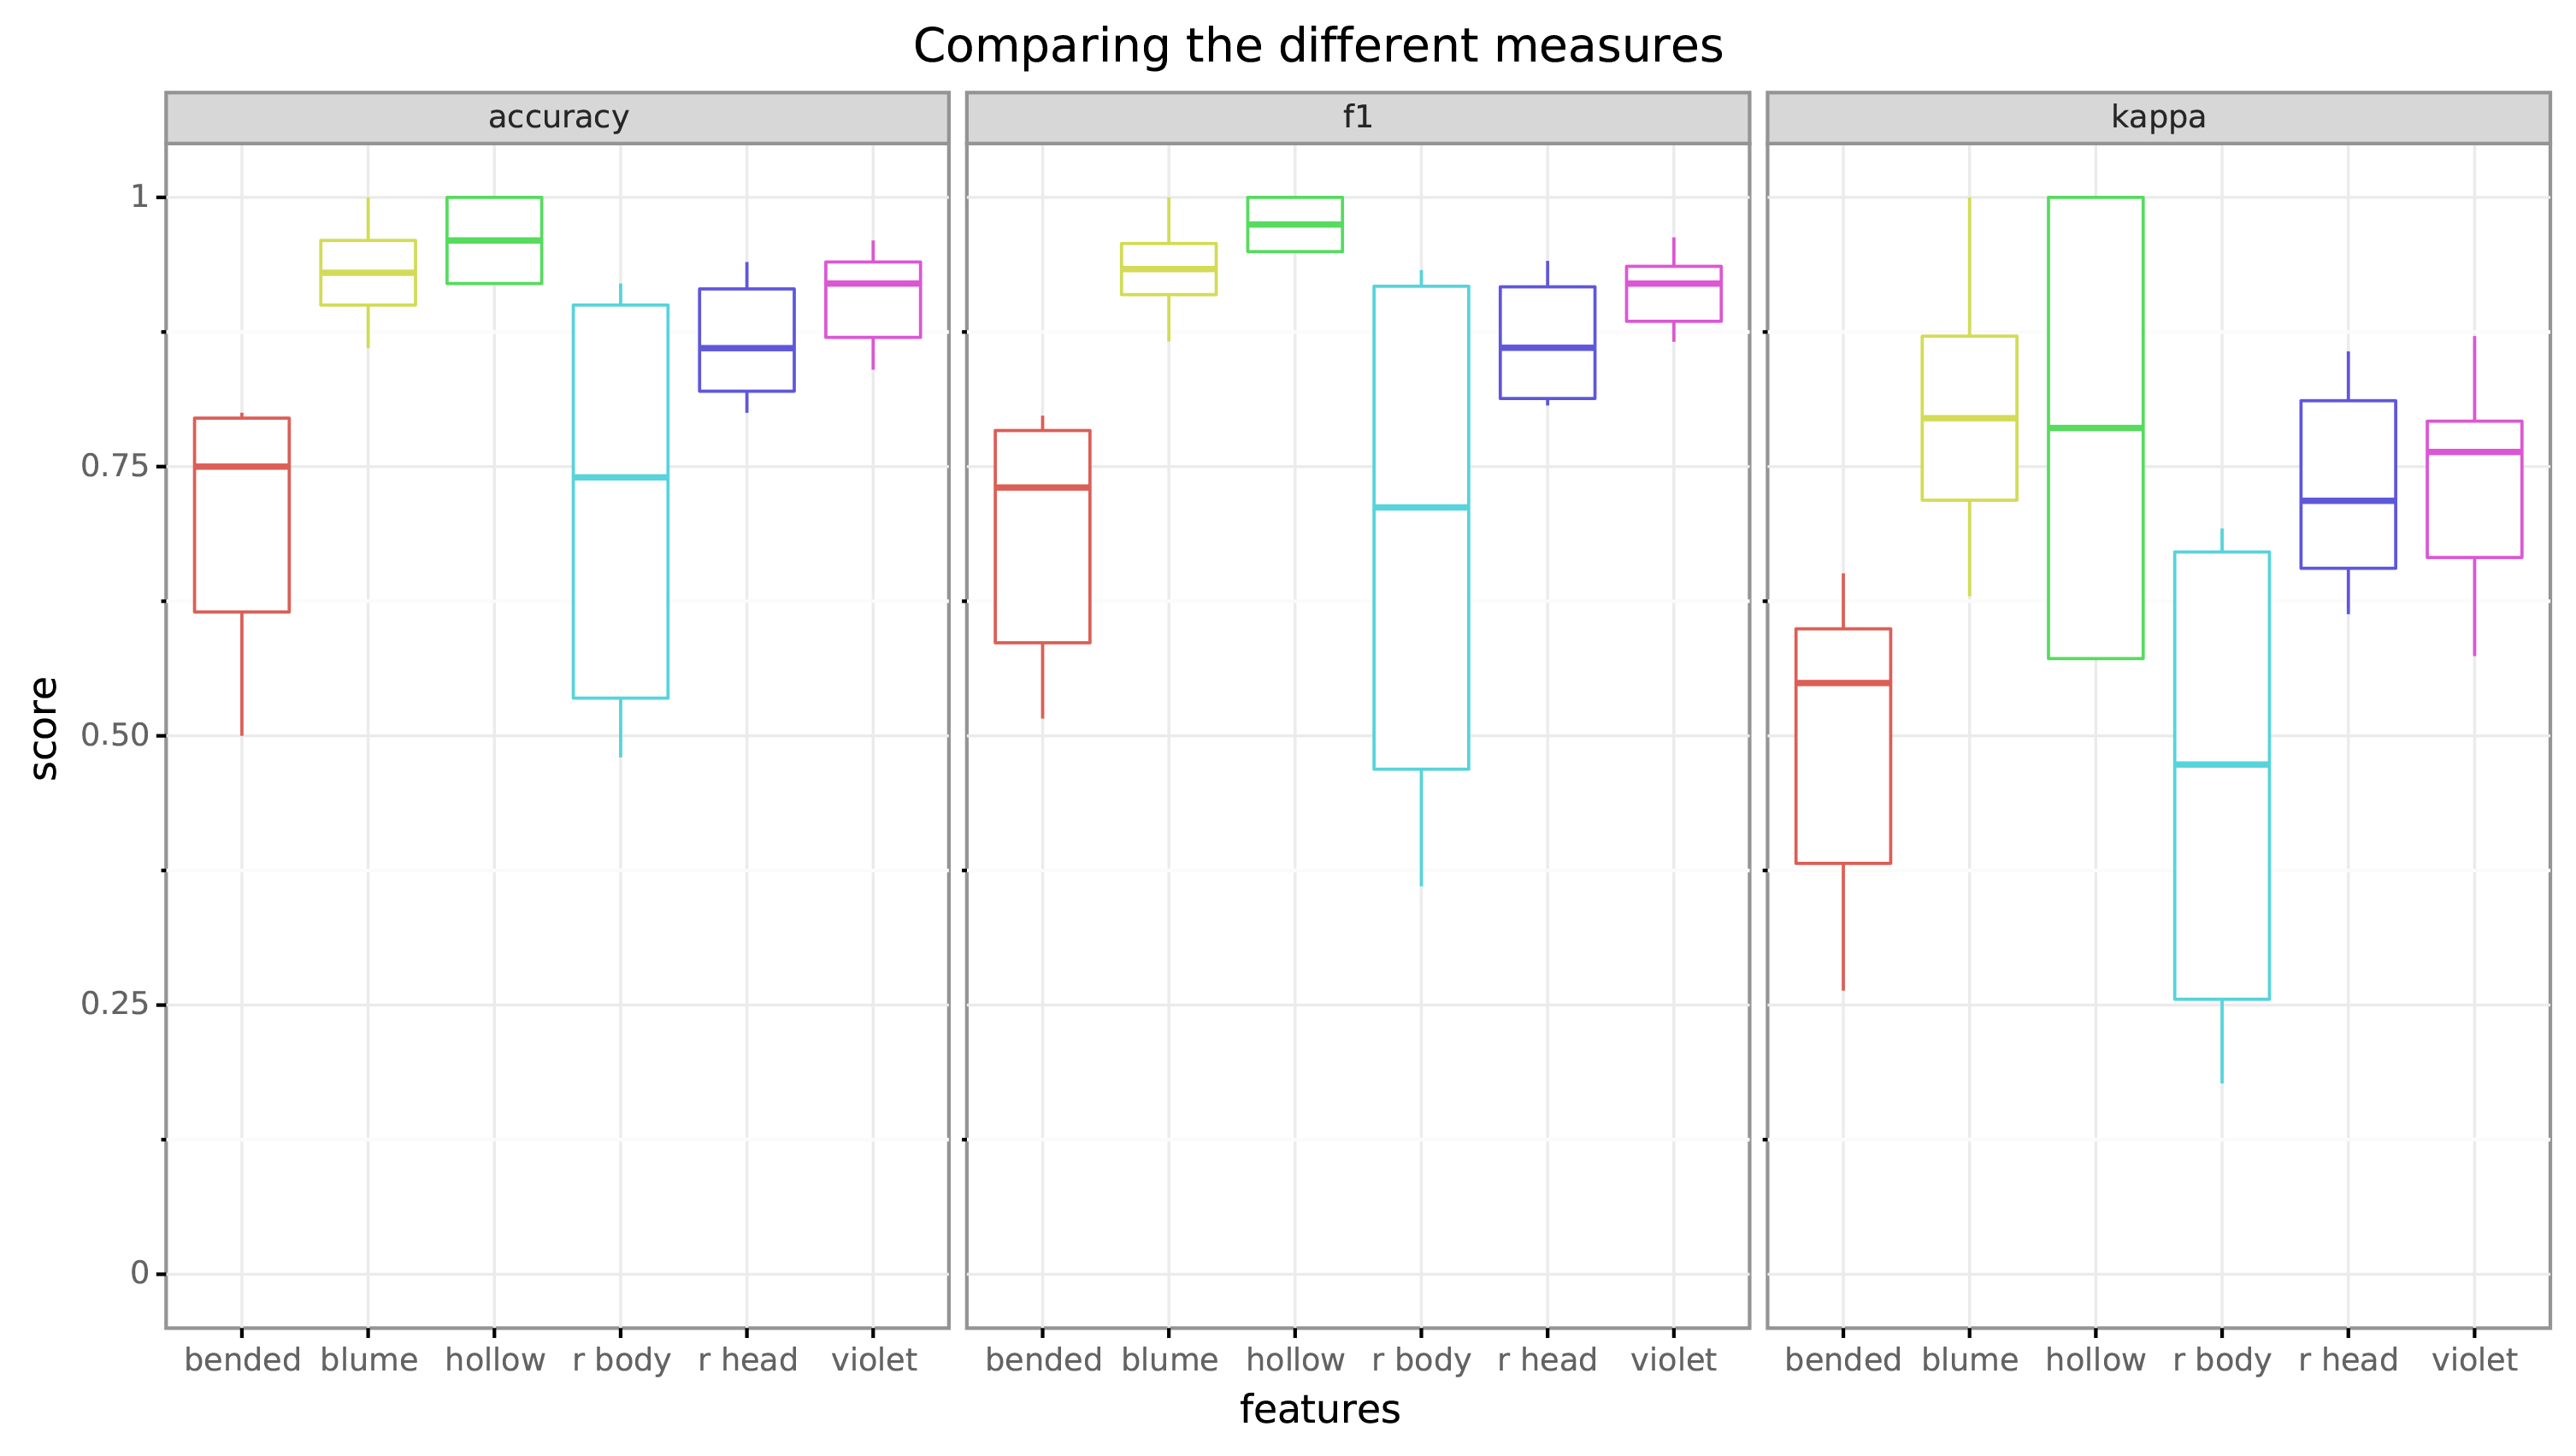
\includegraphics[scale=0.55]{Figures/chapter03/kappa_measurewise.png}
	\decoRule
	\caption[Agreement Measure-Wise Comparison of all Features]{\textbf{Comparing Measures}~~~The figure shows the agreement measures accuracy, F1 and Cohen’s Kappa, separately for each manually labelled feature. Shown are the box-plots, so the middle line indicates the median, the box indicates the IQR. All scores are aggregated scores over all annotator pairs.}
	\label{fig:KappaMeasurewise}
\end{figure}

\begin{figure}[!ht]
	\centering
	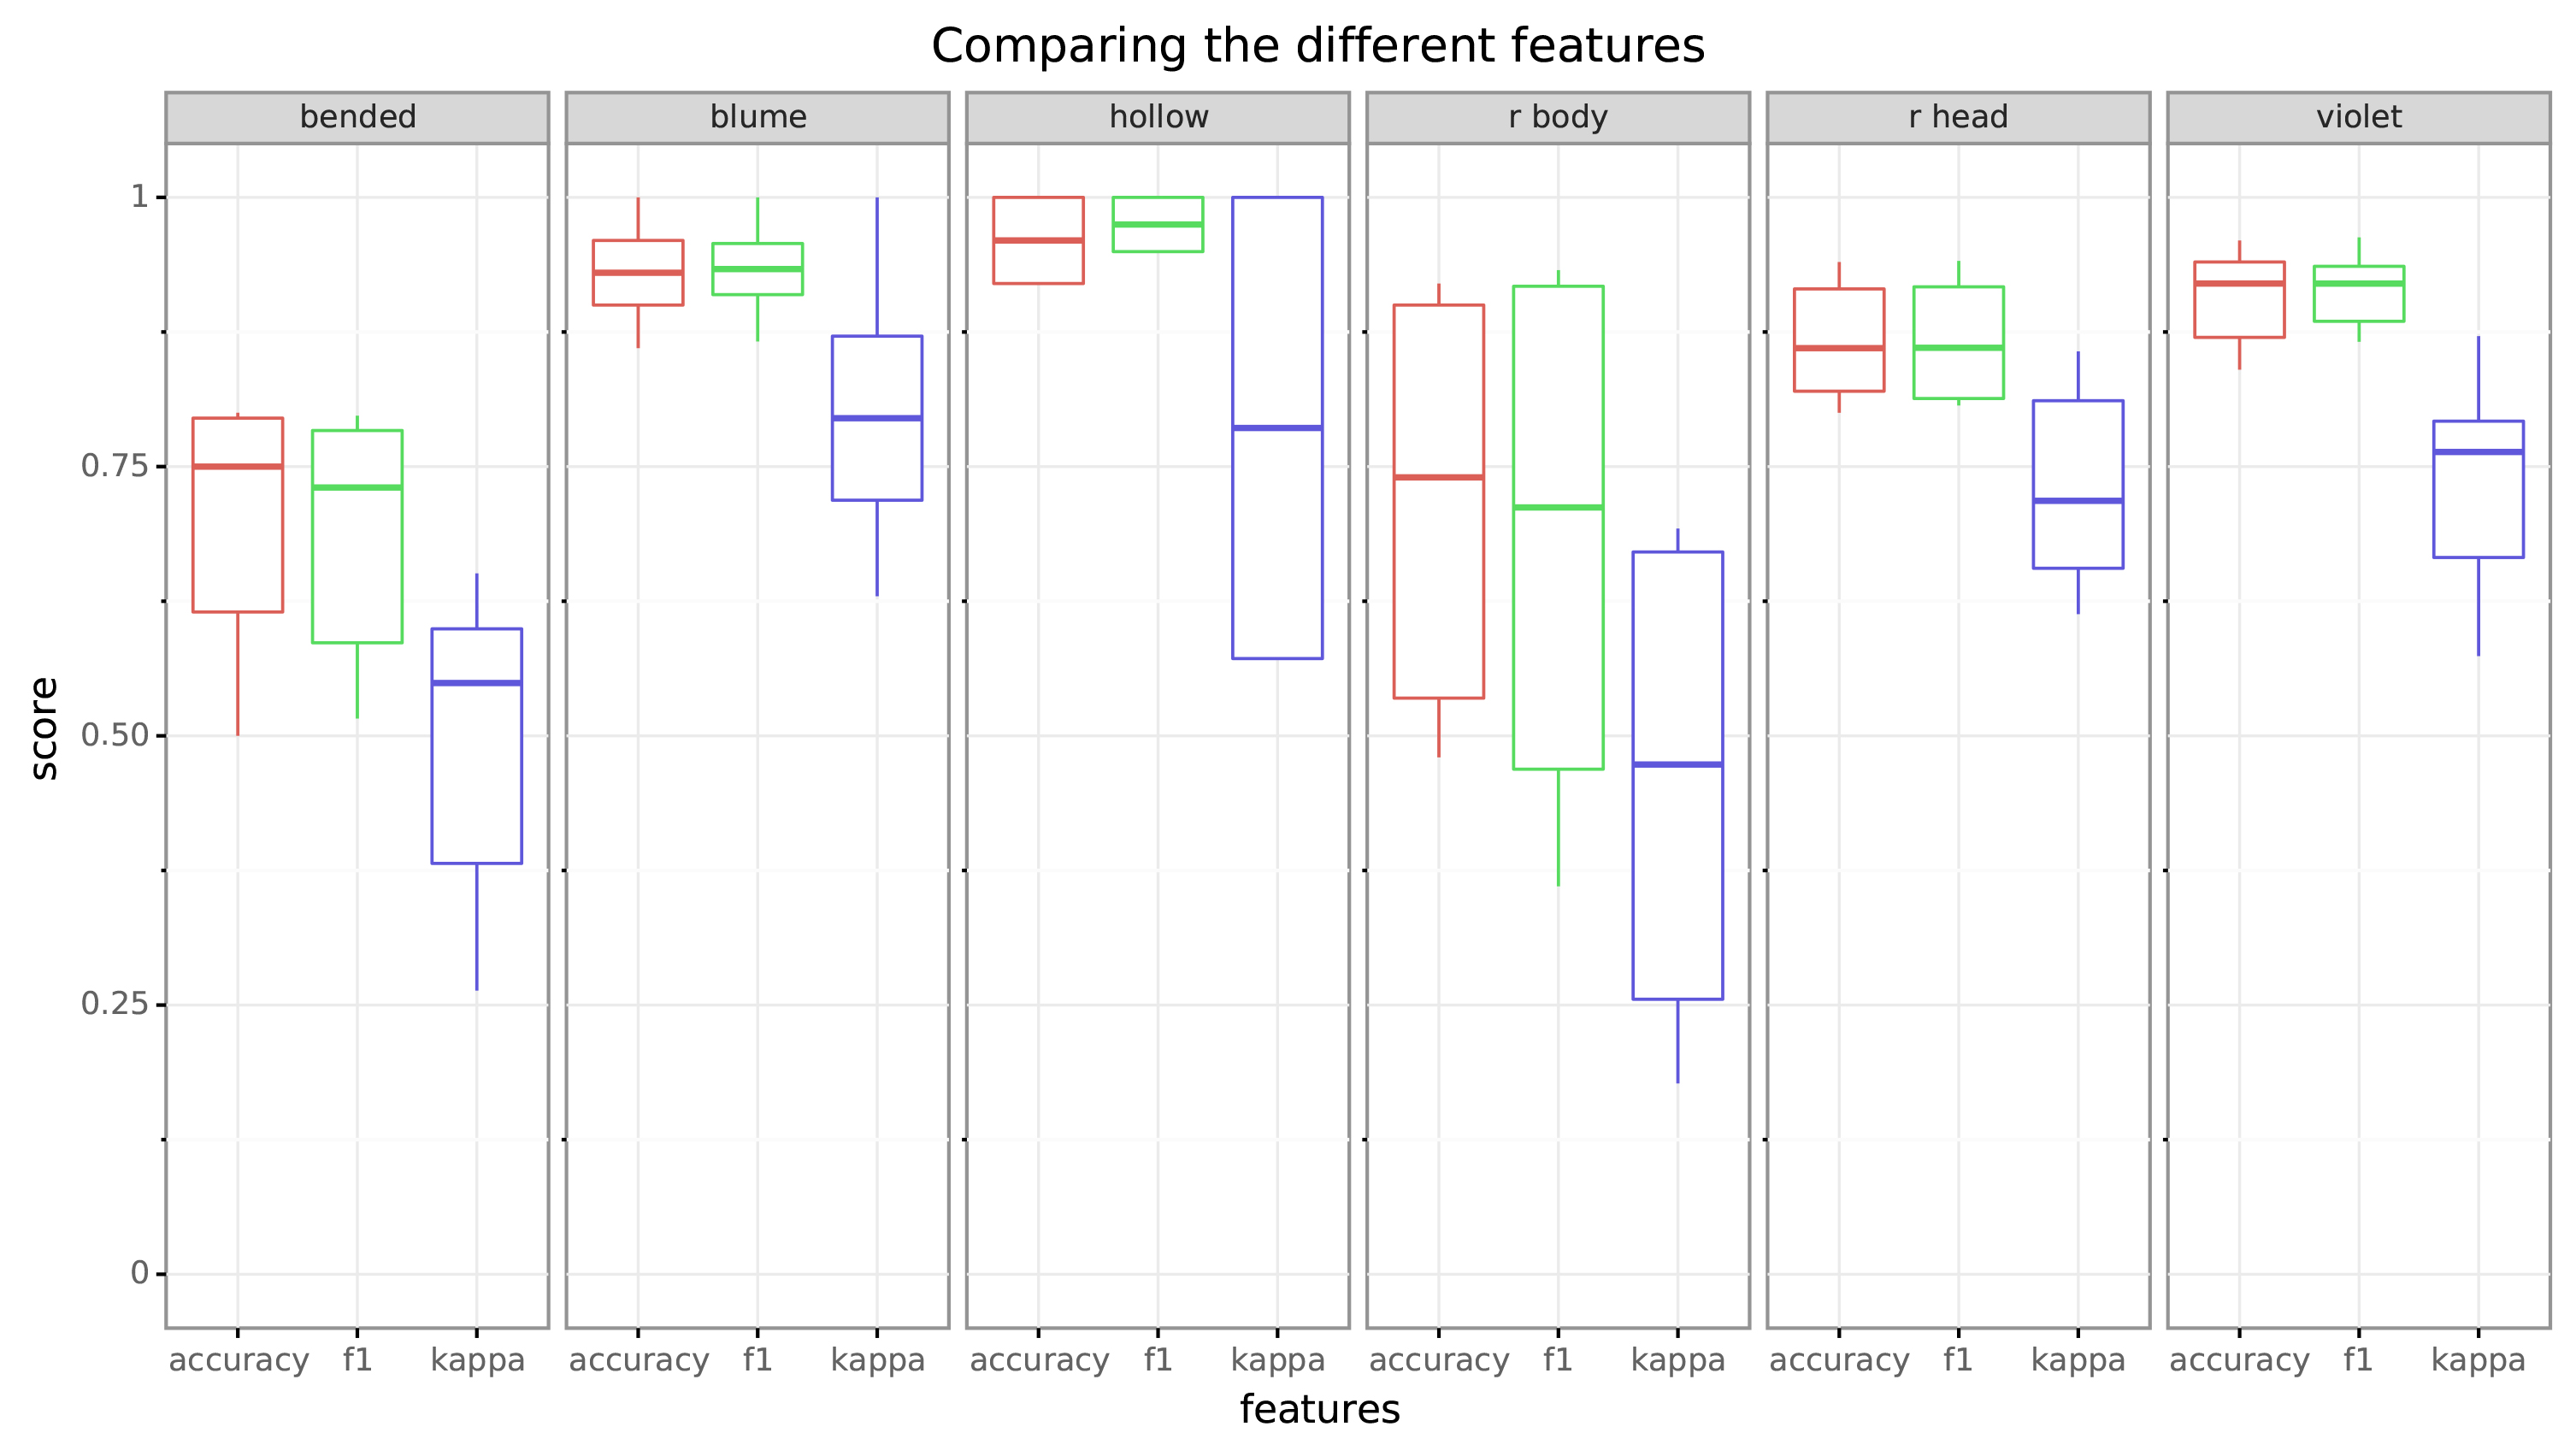
\includegraphics[scale=0.55]{Figures/chapter03/kappa_featurewise.png}
	\decoRule
	\caption[Feature-Wise Comparison of Agreement Measure Scores]{\textbf{Comparing Features}~~~The figure shows each feature separately. For each feature, the corresponding accuracy, F1 and Cohen’s Kappa score is given. Shown are the box-plots, so the middle line indicates the median, the box indicates the IQR. All scores are aggregated scores over all annotator pairs.}
	\label{fig:KappaFeaturewise}
\end{figure}

One reason for our results could be that we compared the agreement class-wise. The occurrence of 1s and 0s per class is therefore very unbalanced. For Kappa scores, if the distribution of 0s and 1s is not balanced, disagreement of the underrepresented value is punished more heavily.\footnote{see also \\ \url{https://stats.stackexchange.com/questions/47973/strange-values-of-cohens-kappa}} Therefore, we decided to repeat our agreement measure feature-wise on non-labeled images, so that the annotators cannot anticipate a specific group label. In order to better understand the reliability of our data, we additionally decided to look at the accuracy score and the F1 score.  Beforehand, the team labeled another 50 images all together, clarified classification boundaries again and discussed unclear images.

The second time, 50 images were labeled by four annotators. The agreements were measured annotator-pair-wise, and then averaged. The results in the Cohen’s Kappa score vary between and within features, and between annotator pairs as well. The highest aggregated kappa score over all annotator pairs is reached for the features flower (0.79) and hollow (0.79), then violet (0.76), rusty head (0.72), bent (0.55) and lastly for rusty body (0.47).
For the features flower, rusty head and violet, the interquartile range (IQR) is quite small, whereas the IQR for hollow, bent and rusty body is much larger (see \autoref{fig:KappaMeasurewise} and \autoref{fig:KappaFeaturewise}).

The agreement scores accuracy and F1 yield very similar results. Results are slightly better than the Kappa scores, in total and for each feature. The highest median accuracy score is reached for the feature hollow (0.96), then flower (0.93), then violet (0.92), then rusty head (0.86), then bent (0.75) and then rusty body (0.74). The order is the same for the F1 scores. The median F1 scores lie between (0.71 and 0.97).

\bigskip
All in all, it can be said that the agreement scores indicate moderate up to substantial agreement. Regardless of the measurement, agreement is highest for the features flower, violet and rusty head.


\subsection{The asparagus data set}
\label{sec:AsparagusDataSet}

In this section, it is described how the images are processed to generate varying data sets. After giving a theoretical overview of the different possibilities of creating data sets for the TensorFlow framework, a description of the methods used in practice is given. It is described which common methods are used to prepare and transform the data. Introduced are the methods of simply using raw data, creating a numpy file, saving a Tensor or a \texttt{TFRecord} file, the \texttt{tf.data} API and the \texttt{tf.data.dataset} API. These methods are compared and followed by a recommendation for further work with the data set.

One question arising in regards to modeling a data set is: What is the best way to provide a model with the input image and corresponding information? The most straight-forward variant is to build the model first, then read in the raw data, and load the samples one after the other. However, the runtime is slow and further processes, which are described below, are not efficient. Additionally, there may be an overflow and large amounts of data do not fit into the memory.

\begin{figure}[!ht]
	\centering
	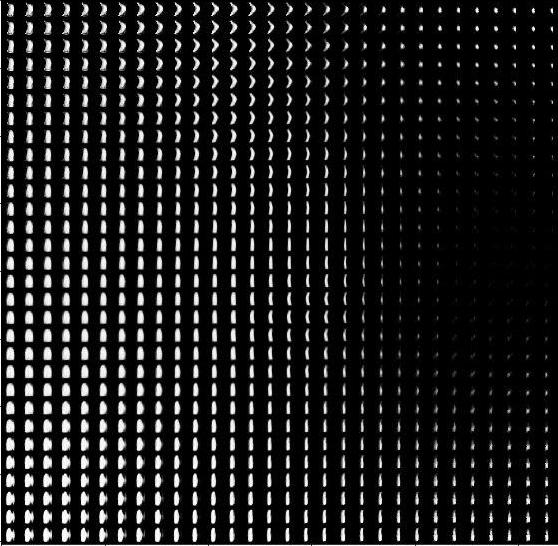
\includegraphics[scale=0.55]{Figures/chapter03/latent-space-square.png}
	\decoRule
	\caption[??]{??}
	\label{fig:LatentSquare}
\end{figure}

\bigskip
One of the used data sets is constructed with all the labeled images in a single numpy array, which can be stored and loaded. As the three perspectives of each asparagus spear are concatenated horizontally, they appear to lie next to each other in the resulting image. These concatenated images are then combined to the final file. The first out of four dimensions in this file depicts the number of labeled asparagus spears. The second and third dimension represent the height and the width of the images, respectively. Further, the fourth dimension represents the three RGB values.
In addition, the images are downscaled to facilitate the training process and reduce memory consumption. Each image is downsampled by a factor of six, that means every 6th pixel is used in the reduced image. This factor can be easily changed and a new data set can be created. 

\bigskip
In the following, TensorFlow's own binary storage format \texttt{TFRecord} is introduced. This approach facilitates the mix and match of data sets and network architectures. The large amount of data that was collected has a significant impact on our import pipeline and, therefore, on the total training time. The file format is optimized for images and text data. These are stored in tuples which always consist of file and label. In our case, the difference in reading time is significant, because the data is stored in the network and not on a SSD on the local PC. The serialized file format allows the data to be streamed efficiently through the network efficiently. Another advantage is that the file is transportable over several systems, regardless of the model one wants to train.

Two data sets are created in this file format. One with all files that were preprocessed, and another one with the preprocessed and labeled data.
The first binary file includes images with background in png format and has a size of 225 Gigabyte (GB). The \texttt{TFRecord} file does not only take up less memory capacity, but can also be read more efficiently. The second data set with all the labels included is reduced in memory space as well.

Working with these ``like lazy list’’-files simplifies the next steps of transformations. With the \texttt{tf.data} API complex, input pipelines from simple and reusable components are created, even for large data sets. The preferred pipeline for our asparagus project can apply complex transformations to the images and combine them into stacks for training, testing and validating in arbitrary ratios. A data set can be changed, e.g.\ by using different labels or by transformations like mapping, repeating, batching, and many others. These dozens of transformations can be combined. A frequently used order is described below. The principle of these ``like lazy list’’ can be found in most mainstream languages like C\#'s LINQ or Java 8's streams.

\bigskip
One frequently used order for the different transformations is:
\begin{enumerate}[noitemsep]
\item create the data set
\item shuffle (with big enough buffer size)
\item map with the actual work (preprocessing, augmentation…) using multiple parallel calls
\item batch
\item prefetch
\end{enumerate}


Besides the described functional transformations of the input pipeline under \texttt{tf.data.dataset}, an iterator gives sequential access to the elements in the data set. The iterator stays at the current position and allows to call the next element as a tuple of tensors. Initializable iterators go through the data set in parallel. In addition, different parameters are passed to start the call. This is especially handy when searching for parameters.

In summary there are two advantages using \texttt{tf.data}. On the one hand, it is possible to build a data set with different data sources. On the other hand, there are many functional transformations and an iterator with sequential access to the data.

\bigskip
Derek Murray recapitulates: ``If you compare a \texttt{tf.data} pipeline to the equivalent queue-based pipeline, we use a similar structure of queues and threads, but importantly there are no Python queue runner threads on the critical path, and so the \texttt{tf.data} pipeline is not constrained by the Global Interpreter Lock and it scales to much higher throughputs.’’~\citep{dataAPI}. 

\bigskip
Further we tried to add our data set to the TFDS~\footnote{see~\url{https://www.tensorflow.org/datasets/beam\_datasets}}. TFDS enables all users to access the data set directly using the TensorFlow API. For this, we need to publish the data. This is possible in terms of data integrity. However, the process of publishing the data set turned out to be too time consuming. Especially the large amount of data was a problem. Questions like: How do we deal with the fact that only a part of the images has labels? How should we pass the labels: each as a feature, in a list, or as several features? It would have been better, faster, and more helpful for the development of the network approaches, if we had continued to search and to integrate the \texttt{TFRecord} files with the \texttt{tf.data} API in our pipeline early. 
